\chapter{Discussion and Recommendations}
\label{cha:disc-recomm}

In this chapter the achieved results are discussed, as well as some tasks that
have not been achieved. \Cref{cha:evaluation} already discussed how the final
product satisfied the client's requirements. This chapter goes more in-depth why
not all these requirements have been met.

Afterwards, some recommendations are made that will further enhance and provide
possible directions for future work on the product.

\section{Discussion}
\label{sec:discuss-discussion}

TODO: section introduction

\subsection{Language interpreters have to be on the classpath}
\label{sec:discuss-classpath}

\subsection{Textual representation of DynSem data types}
\label{sec:discuss-dynsem-string}


%\input{discuss-recommend/disc-eclipse}

\section{Recommendations}
\label{sec:discuss-future}

This section makes several recommendations to the client for future work on the
delivered product. These recommendations come forth from requirements that have
not been implemented (see \cref{ssec:eval-requirements}) and opportunities for
improvements in the delivered product. First, recommendations are made to
improve the REPL backend itself. Secondly, suggestions are made on
how to improve the Eclipse frontend. Finally, recommendations to provide
additional frontend implementations are made.

\subsection{Extending the functionality of the REPL}
\label{ssec:impr-backend}

The delivered backend is a solid product. Due to time constrains, however, some
nice to have features have not been implemented. This subsection shortly
highlights these features.

\subsubsection{More extensive history functionality}

The current input history implementation provides a means of iterating the
previously entered expressions in a linear way: a user can scroll back and forth
through the old entries. It would be nice if the history was searchable, too.
When implementing this, one could turn to existing command-line shells for
inspiration. The GNU readline library, for example, has two ways of searching
through the input history: via a keyboard shortcut, which when pressed allows
the user to enter a word that they remember is in the entry they are looking
for, or via an always-on setting that allows the user to enter the beginning of
the expression which will in turn filter the linear iteration over the
history to only those entries starting with the entered input.

Another limitation of the current history implementation is the fact that it is
recorded per session. This means that when a user uses several languages in the
same session, the history will contain entries from both languages. Instead,
history should perhaps be kept not only per session, but also per language.

Related to the above, is implementing persistent history. The Eclipse frontend
currently only provides volatile history, which means that history is thrown
away when Eclipse is closed. The console plugin does provide persistent history,
but this implementation also leaves things to be desired: all history is saved
into the same file, resulting again in a mixed history. The recommendation that
is made here is to provide the ability to have separate, per language
persistent history. If the frontend is an IDE, these files can perhaps be saved
inside the language project's directory structure.

Improving the history implementation should result in a smoother and
faster way to interact with the REPL, enhancing the explorative nature.

\subsubsection{Analysis in context}

%%% Local Variables:
%%% mode: latex
%%% TeX-master: "../main"
%%% End:


\subsubsection{Adding support for alternative evaluation strategies}
\label{ssec:discuss-alternate-eval}

As discussed in \cref{sec:eval-strat}, languages developed with Spoofax are not
limited to a single interpreter. Instead, there can be different strategies for
evaluation. While this has been taken into account for the design of the
product, only a DynSem evaluation strategy has actually been implemented.

Languages with a Java backend (such as IceDust%
\footnote{https://github.com/MetaBorgCube/IceDust}) therefore do not currently
work with the REPL. To add support for specific interpreters, a language should
provide the REPL with a named implementation of the
\texttt{``IEvaluationStrategy''}. The language designer can register alternative
evaluation strategies with the REPL by extending the Guice module of the backend
and overriding the \texttt{bindEvalStrategies} method.

Finally, the evaluation strategy that will be used to evaluate input terms can
be configured via the ShellFacet ESV extensions (see \cref{sec:esv-extensions})
as illustrated in \cref{lst:eval-method}.

\begin{lstlisting}[language=esv,caption={Setting the evaluation strategy.},label={lst:eval-method}]
module editor/SL-Shell

shell
    evaluation method : "dynsem"
\end{lstlisting}



\subsection{Improvements to the Eclipse frontend}
\label{ssec:impr-eclipse}

The Eclipse frontend that is delivered with the product has been discussed in
\cref{ssec:eclipse-plugin}. The plugin provides interaction with the REPL
backend, as discussed in \cref{chap:design}.

The delivered Eclipse frontend is just that: a frontend to the REPL backend.
Integration with Eclipse and Spoofax Eclipse are not yet present. This
subsection provides several recommendations to better integrate this frontend
into Eclipse and Spoofax Eclipse.

\subsubsection{Building languages and projects}

TODO: write this when the discussion on classpath issues has been written.
Mention that there should be a button to build the language/project, put it on
the classpath and launch it in a REPL.

\subsubsection{Back and forth interaction between Eclipse and the REPL}

A feature the REPL does not yet support is loading existing files into the
evalution context (see \cref{ssec:discuss-repl}). When it does, this interaction
could provide deeper integration between the REPL and Spoofax Eclipse. For
example, hovering over variables could indicate from where they originate, or
changes in a currently loaded file could be automatically picked up. Changes in
the other direction are interesting, too: when a loaded function is overridden
inside the REPL, an option could be provided to apply this change to the loaded
file as well.

\subsubsection{Improving the UI of the Eclipse REPL}

The user interface currenty offered by the Eclipse frontend does not resemble a
typical REPL: the input and output views are separated. To improve the user
experience, these two views could be merged into one. TODO: expand and give
pointers as to how this might be possible?

TODO: recommend missed features such as autocompletion et cetera?

%%% Local Variables:
%%% mode: latex
%%% TeX-master: "../main"
%%% End:


\subsection{Alternative Frontend Implementations}
\label{ssec:discuss-alternative-frontend}

\Cref{sec:frontends} showed that implementing different frontends is
straightforward: only a handful of interfaces have to be implemented in order to
provide a basic frontend. The client has expressed their interest in numerous
other frontends, which have not been implemented due to time contraints.
However, because providing additional implementations is straightforward,
several recommendations for additional frontends are made in this subsection.

\subsubsection{An IntelliJ Frontend}
\label{ssec:intellij}

As has been said before, an effort is currently underway to provide different
IDE-implementations of Spoofax. The Spoofax for IntelliJ IDEA
project\footnote{See:
\url{http://metaborg.org/en/latest/source/langdev/manual/env/intellij/}}
provides a plugin for the IntelliJ IDEA IDE. The client has expressed their
interest in having the REPL available in this IDE as well.

This IntelliJ IDEA REPL would then provide the same features as the current
console- and Eclipse REPLs.

%%% Local Variables:
%%% mode: latex
%%% TeX-master: "../main"
%%% End:


\section{Literate Programming}
\label{sec:literate-programming}

Just as with REPLs, the concept of literate programming is implemented in
various forms under various names. Therefore, this section starts with an
explanation of what literate programming is based on a few implementations.
Afterwards, the IPython implemention of literate programming is explored in more
detail.

Literate programming, as defined by Donald Knuth~\cite{knuth1984}, introduces
the ability to annotate source code with natural language. According to Knuth,
better documentation of programs is essential to make further progress in the
state of the art of programming.  To achieve this he proposes to write programs
not with the intention to explain the computer what to do, but with the
intention to explain to humans what the programmer wants a computer to
do~\cite{knuth1984} by mixing documentation and source code in a single file.
This idea of literate programming was realized in its original form as the
``WEB'' language developed during Knuth's research at Stanford University.

Even though the idea was conceived over thirty years ago, implementations are not
very common. However, in recent years the idea seems to gain popularity again.
A very recent implementation of literate programming is Apple's Swift
playgrounds~\cite{swift-playgrounds}. Swift playgrounds are interactive
documents or ``notebooks'' in which code is executed as it is typed, in
contrast to the non-interactive style of the ``WEB'' language in which \TeX{} and
PASCAL were combined into one language: \TeX{} served to document the program
and PASCAL to produce a machine-executable program.

In recent years, there has also been a particular focus on reproducible
research. While literate programming primarily aims to add documentation to
code, reproducible research focuses on adding code to documentation. More
specifically, reproducible research refers to the idea that scientific papers
should be augmented with the computer code used to carry out the
research~\cite{schulte2012}. Examples of recent projects claiming to support
both reproducible research and literate programming include the IPython
project~\cite{ipython2007} and Emacs Org-mode~\cite{schulte2012}.

\subsubsection{IPython with Jupyter notebooks}

IPython, together with Jupyter notebooks,
supports both reproducible research and literate programming. IPython was
partially inspired by other scientific tools already offering notebook-like
functionality, such as Matlab or Mathematica. Since its inception, the project
has been split off into IPython, which provides an interactive REPL and a
kernel that runs the user's code, and Jupyter notebooks, which provide the
notebook format and web application. Like Swift playgrounds, Jupyter notebooks
allow for REPL-style interactive editing; documentation and code can be edited
live and blocks of code can be reevaluated, printing their updated results.
Jupyter notebooks also allow for more complex graphical elements such as
3D-plots. See \cref{fig:ipython} for an example of an IPython notebook.

\begin{figure}[htb]
  \centering
  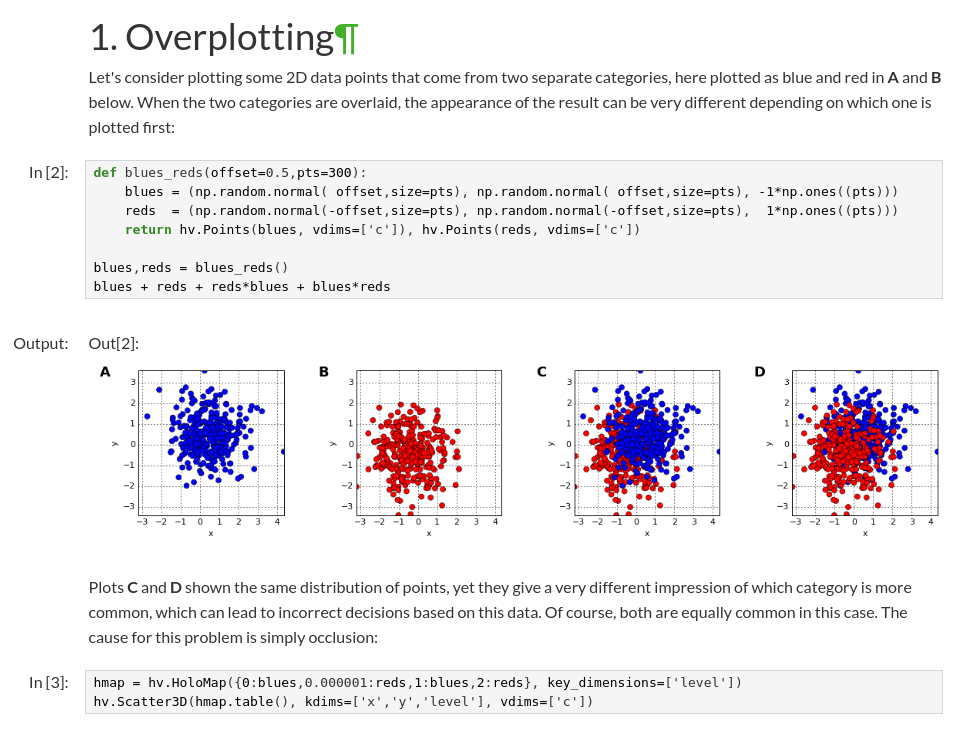
\includegraphics[width=\textwidth]{ipython}
  \caption{A plot from data in an IPython notebook.}
  \label{fig:ipython}
\end{figure}

As explained, IPython and Jupyter notebooks have become more or less separate
projects, to the extent that Jupyter notebooks can use several kernels.
Nowadays there are kernels for over forty languages that can be used in these
notebooks. This illustrates that in Python's case literate programming is more
or less an extension to the interactive IPython REPL. Since Jupyter notebooks
reuse the IPython REPL, the execution model used for Jupyter notebooks is
essentially the same as it is for IPython~\cite{ipython-execution}.

%%% Local Variables:
%%% mode: latex
%%% TeX-master: "../main"
%%% End:


%%% Local Variables:
%%% mode: latex
%%% TeX-master: "main"
%%% End:
